\ATLAS\ includes two types of calorimeter systems, the Liquid Argon calorimeter (LAr) and the Tile calorimeter (TileCal) for measuring electromagnetic and hadronic showers respectively.
Together, these cover a region of $|\eta| < 4.9$.
A cut away view of the calorimeter system can be seen in Figure \ref{fig:detector:calorimeters}.
\begin{figure}[ht]
  \begin{center}
    \makebox[\textwidth][c]{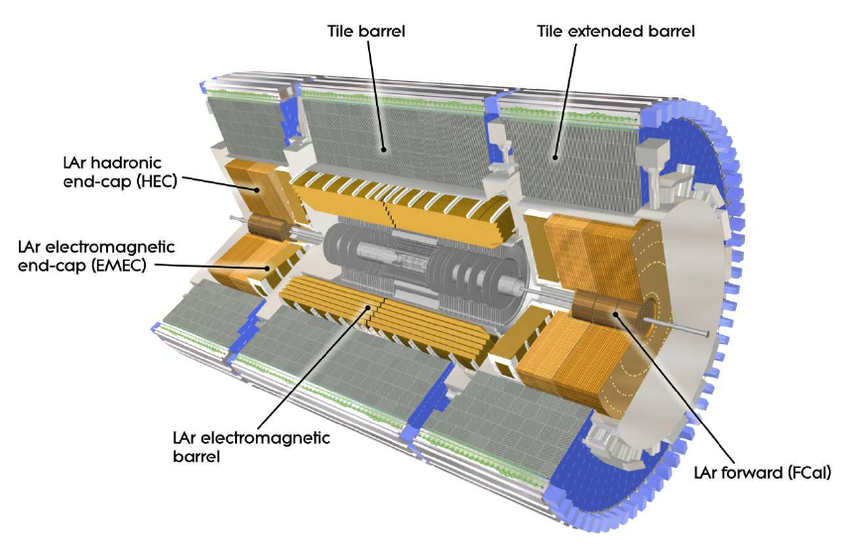
\includegraphics[width=0.92\textwidth]{figs/detector/Cut-away-view-of-the-ATLAS-calorimeters-The-LAr-calorimeters-are-seen-inside-the.png}}
  \end{center}
  \caption[Cut-away view of the ATLAS calorimeters. The LAr calorimeters are seen inside the hadronic Tile  calorimeters]
          {Cut-away view of the ATLAS calorimeters. The LAr calorimeters are seen inside the hadronic Tile  calorimeters \cite{PERF-2007-01}.}
  \label{fig:detector:calorimeters}
\end{figure}

\subsubsection{Liquid Argon Calorimeters} 
\label{sec:lar}
The EM calorimeter is a lead/liquid-argon (LAr) sampling calorimeter with an accordion geometry made up of layers of passive Pb absorber alternating with active liquid argon detector layers.
As and electron or a positron or photon passes through the absorber the particle will cascade electromagnetically: photons produce electron-positron pairs and electrons/positrons will emit bremsstrahlung photon radiation; the daughter electrons, positrons, and photons also interact, resulting in a particle shower.
Most of the energy will have been absorbed after traversing about 20 radiation lengths ($X_{0}$) of absorber (longitudinal depth).
Note that lead has a radiation length of only 0.56 cm so the electromagnetic calorimeter is able to be rather compact at 53~cm (62~cm) deep in the barrel (endcap).
The lateral width of the shower in a material is characterized by its Moli\'ere radius, the radius of a cone in which 90\% of the shower energy is contained.
Note that lead has a Moli\'ere radius of only 1.6~cm, so the energy deposits in the calorimeter from electrons, positrons, and photons have a very narrow width in the detector.
This is a key for identification of electrons.
\begin{figure}[h]
  \begin{center}
    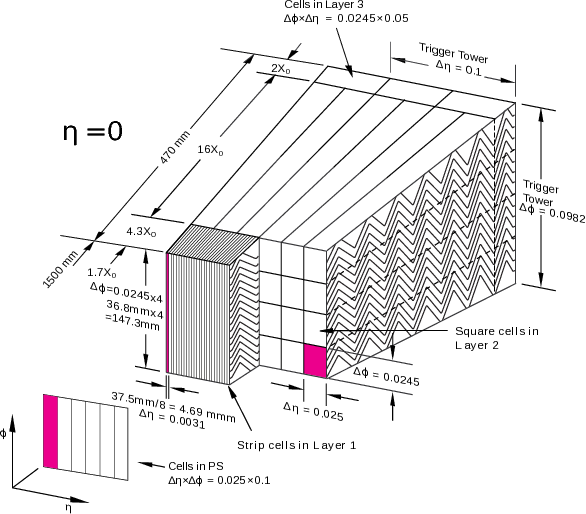
\includegraphics[width=0.92\textwidth]{figs/detector/LAR.png}
  \end{center}
  \caption[Illustration of the LAr calorimiter detailing the different granularities and radiation lengths of each layer]
          {Illustration of the LAr calorimiter detailing the different granularities and radiation lengths of each layer \cite{PERF-2007-01}.}
          \label{fig:detector:LAr}
\end{figure}

The calorimeter is divided into a barrel section (EMB) covering the pseudorapidity region $|\eta|<$ 1.475, and two endcap sections (EMEC) covering 1.375 $<|\eta|<$ 3.2.
The barrel and endcap calorimeters are immersed in three LAr-filled cryostats, and are segmented into three layers for $|\eta|<$ 2.5.
The layered and accordion structure of the LAr are illustrated in Figure~\ref{fig:detector:LAr}, showing a section of the barrel LAr calorimeter.
Layer 1 covers $|\eta|<$  1.4 and 1.5 $<|\eta|<$ 2.4, has a thickness of about 4.3 radiation lengths ($X_{0}$) and is finely segmented in the $\eta$ direction, typically 0.003 $\times$ 0.1 in $\Delta \eta \times \Delta \phi$ in the EMB, to provide discrimination between electromagnetic showers initiated by a single electron or photon and those initiated by the two photons from the decay of a neutral pion~\cite{PERF-2007-01}.
Layer 2, which collects most of the energy deposited in the calorimeter by electromagnetic showers, has a thickness of about 17~$X_{0}$ and a granularity of 0.025 $\times$ 0.025 in $\Delta \eta \times \Delta \phi$ \cite{PERF-2007-01}.
Layer 3, which has a granularity of 0.05 $\times$ 0.025 in $\Delta \eta \times \Delta \phi$ and a depth of about 2$X_{0}$, is used to correct for leakage beyond the EM calorimeter for high-energy showers \cite{PERF-2007-01}.
In front of the accordion calorimeter, a thin presampler layer (PS) covering the pseudorapidity interval $|\eta|<$ 1.8, is used to correct for energy loss upstream of the calorimeter.
The PS consists of an active LAr layer with a thickness of 1.1 cm (0.5 cm) in the barrel (endcap) and has a granularity of $\Delta \eta \times \Delta \phi$ = 0.025 $\times$ 0.1.
The transition region between the EMB and the EMEC, 1.37 $<|\eta|<$ 1.52, has a large amount of passive material (from cables and services to the inner detector) in front of the first active calorimeter layer ranging from 5 to almost 10$X_{0}$ \cite{PERF-2007-01}.
This section is instrumented with scintillators located between the barrel and endcap cryostats, and extending up to $|\eta|$ = 1.6.
Note that this transition region is specifically separated in the electron ID due to the lack of precise information available. 
This allows an analyzer to veto the region entirely which is common practice. 

\subsubsection{Tile Calorimeter}
%\textcolor{red}{\hrulefill \textsc{Unfinished Section}\hrulefill}  \\
The main function of the Tile Calorimeter (TileCal) is to contribute to the energy reconstruction of the jets produced in the proton-proton interactions and, with the addition of the end-cap and forward calorimeters, to provide a good \met\ measurement~\cite{ATLAS:1996aa}.
The TileCal surrounds the EM calorimeter and extends radially from 2280~mm to radius of 4230~mm.
It consists of three large segments in as can be seen in Figure~\ref{fig:detector:TileCal}.
The middle segment consists of an alternating iron/scintillator material tile calorimeter with barrel coverage $|\eta|<$ 1.7.
The two outer segments, known as the hadronic end cap (HEC), instead use copper for their absorber and LAr for the active material, spanning 1.5 $ < |\eta| < $ 3.2.
Figure~\ref{fig:detector:TileCal} also illustrates the wedge based module structure of the TileCal. 
The acceptance is extended by two copper/LAr and tungsten/LAr forward calorimeters covering 3.1$<|\eta|<$ 4.9, and hosted in the same cryostats as the EMEC.
\begin{figure}[h]
  \begin{center}
    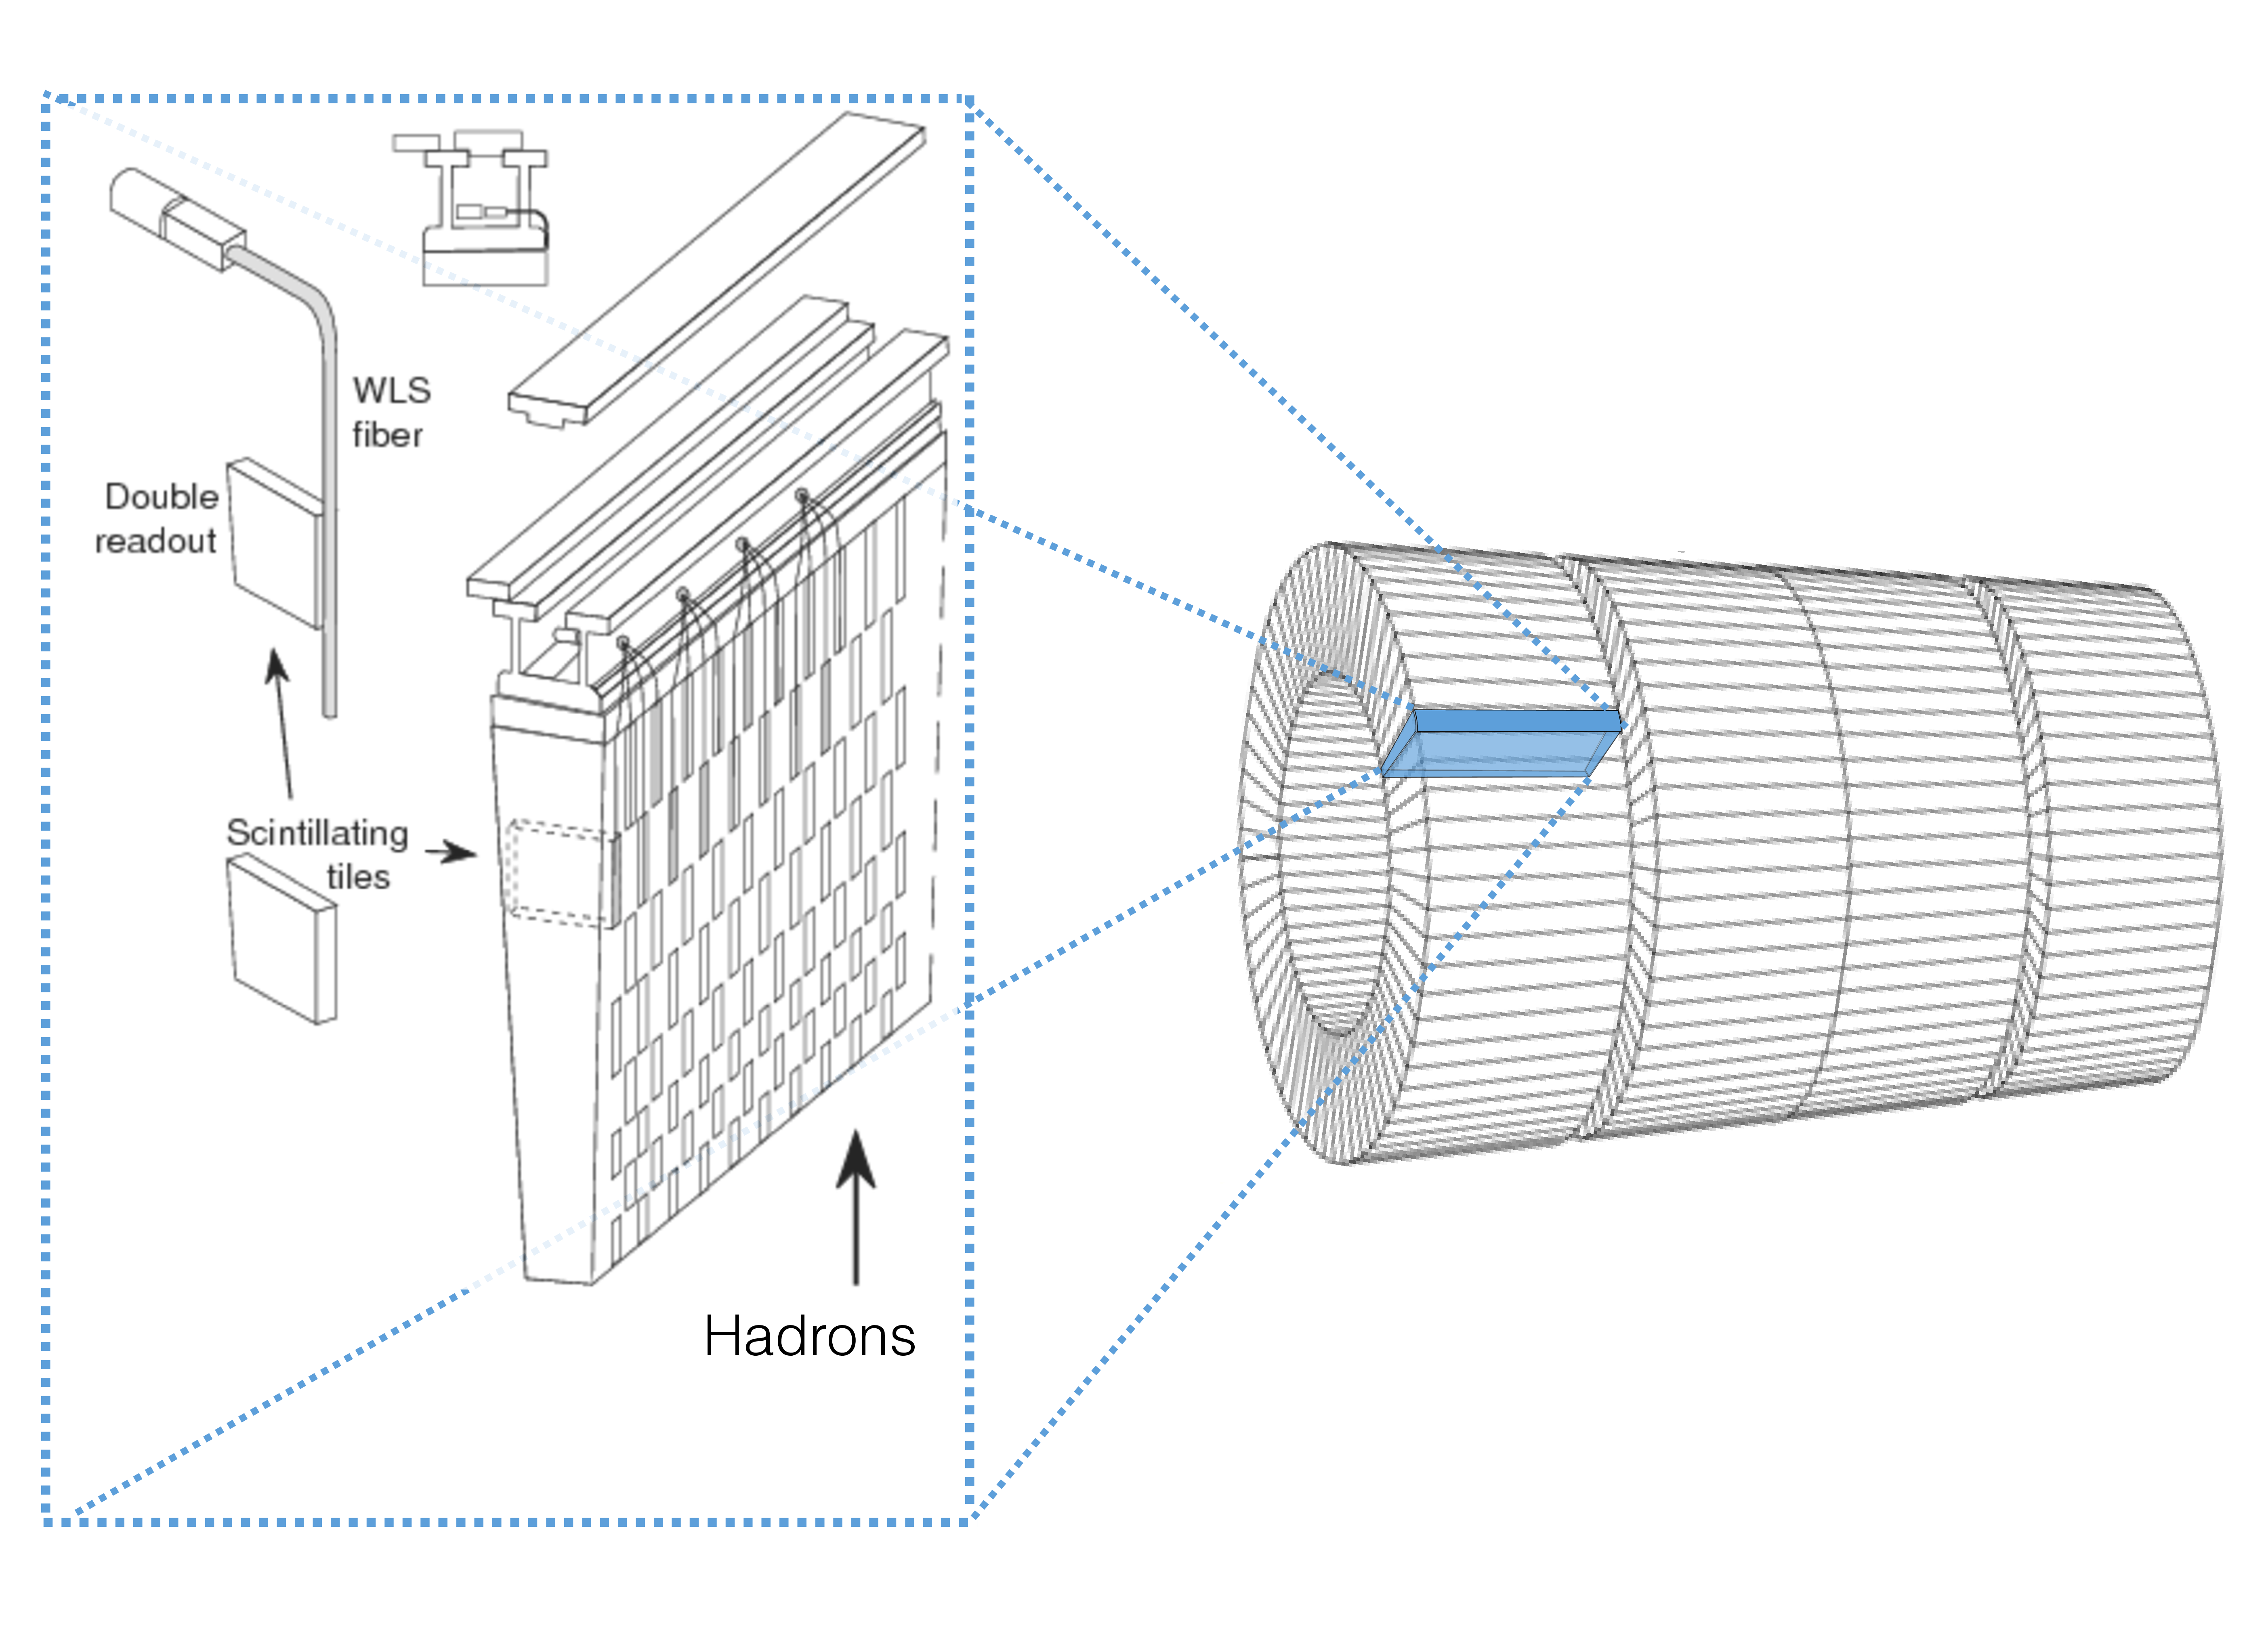
\includegraphics[width=0.94\textwidth]{figs/detector/tilecal.png}
  \end{center}
  \caption[Illustration of the Tile Calorimeter]
          {Illustration of the Tile Calorimeter showing its barrel and end cap segments along with a zoomed-in view of a wedge module diagramming the placement and orientation of the tiles and read out material for one of the HEC segments. Note for the barrel segment the tile orientation is such that its length dimension is along the z-axis instead.}
          \label{fig:detector:TileCal}
\end{figure}